%% This is file 'yjvci-template.tex',
%% 
%% 
%% This file is part of the 'Elsarticle Bundle'.
%% ---------------------------------------------
%% 
%% It may be distributed under the conditions of the LaTeX Project Public
%% License, either version 1.2 of this license or (at your option) any
%% later version.  The latest version of this license is in
%%    http://www.latex-project.org/lppl.txt
%% and version 1.2 or later is part of all distributions of LaTeX
%% version 1999/12/01 or later.
%% 
%% The list of all files belonging to the 'Elsarticle Bundle' is
%% given in the file `manifest.txt'.
%% 
%% Template article for Elsevier's document class `elsarticle'
%% with harvard style bibliographic references
%%
%% $Id: yjvci-template.tex 139 2018-09-06 09:45:00Z rishi $
%% $URL: http://lenova.river-valley.com/svn/elsarticle/trunk/yjvci-template.tex $
%%
%% Use the option review to obtain double line spacing
%\documentclass[times,review,preprint,authoryear]{elsarticle}

%% Use the options `twocolumn,final' to obtain the final layout
%% Use longtitle option to break abstract to multiple pages if overfull.
%% For Review pdf (With double line spacing)
%\documentclass[times,twocolumn,review]{elsarticle}
%% For abstracts longer than one page.
%\documentclass[times,twocolumn,review,longtitle]{elsarticle}
%% For Review pdf without preprint line
%\documentclass[times,twocolumn,review,nopreprintline]{elsarticle}
%% Final pdf
\documentclass[times,twocolumn,final]{elsarticle}
%%
%\documentclass[times,twocolumn,final,longtitle]{elsarticle}
%%

%% Stylefile to load YJVCI template
\usepackage{yjvci}
\usepackage{framed,multirow}

\usepackage{booktabs} % �ṩ���߱�����
\usepackage{amssymb}  % �ṩ \checkmark ����
\usepackage{algorithm}
\usepackage{algpseudocode}
\usepackage{amsmath}
% \usepackage{booktabs} 

%% The amssymb package provides various useful mathematical symbols
\usepackage{amssymb}
\usepackage{latexsym}

% Following three lines are needed for this document.
% If you are not loading colors or url, then these are
% not required.
\usepackage{url}
\usepackage{xcolor}

\usepackage{hyperref}

\definecolor{newcolor}{rgb}{.8,.349,.1}

\journal{Journal of Visual Communication and Image Representation}

\begin{document}

\verso{Given-name Surname \textit{et~al.}}

\begin{frontmatter}

  \title{Salient Object Detection Enhanced Pseudo-Labels
    For Weakly Supervised Semantic Segmentation\tnoteref{tnote1}}%
  \tnotetext[tnote1]{This is an example for title footnote coding.}

  \author[1]{Given-name1 \snm{Surname1}\corref{cor1}}
  \cortext[cor1]{Corresponding author:
    Tel.: +0-000-000-0000;
    fax: +0-000-000-0000;}
  \author[1]{Given-name2 \snm{Surname2}\fnref{fn1}}
  \fntext[fn1]{This is author footnote for second author.}
  \author[2]{Given-name3 \snm{Surname3}}
  %% Third author's email
  \ead{author3@author.com}
  \author[2]{Given-name4 \snm{Surname4}}

  \address[1]{Affiliation 1, Address, City and Postal Code, Country}
  \address[2]{Affiliation 2, Address, City and Postal Code, Country}

  \received{1 May 2013}
  \finalform{10 May 2013}
  \accepted{13 May 2013}
  \availableonline{15 May 2013}
  \communicated{S. Sarkar}

  \begin{abstract}
    %%%
    This paper addresses the limitations of generating pseudo-labels based on Class
    Activation Maps (CAM) in weakly supervised semantic segmentation tasks by
    proposing a novel salient object fusion framework. This framework complements
    CAM localization information by capturing complete contours and edge details of
    salient targets through the designed RGB-SOD network. We also designed a
    saliency object selector to dynamically balance the weights of CAM and SOD when
    generating single-class pseudo-labels, further improving the quality of
    pseudo-labels. Despite its simplicity, our method achieved competitive
    performances of 77.52\% and 77.73\% on the PASCAL VOC 2012 validation and test
    sets respectively, significantly enhancing the performance bottlenecks of
    existing methods. This work highlights the importance of effectively
    integrating complementary information to improve weakly supervised segmentation
    tasks.
    %%%%
  \end{abstract}

  \begin{keyword}
    %% MSC codes here, in the form: \MSC code \sep code
    %% or \MSC[2008] code \sep code (2000 is the default)
    \MSC 41A05\sep 41A10\sep 65D05\sep 65D17
    %% Keywords
    \KWD Keyword1\sep Keyword2\sep Keyword3
  \end{keyword}

\end{frontmatter}

%\linenumbers

%% main text
\section{Introduction}
\label{sec1}

Semantic segmentation is a fundamental task in computer vision that aims to
assign a class label to each pixel in an image. It has been widely applied in
various fields, such as autonomous driving, medical imaging, and scene
understanding. Recently, deep learning-based methods have achieved remarkable
success in semantic segmentation tasks, especially fully supervised methods
that require pixel-level annotations for training. However, obtaining
pixel-level annotations is labor-intensive and time-consuming, which limits the
scalability of fully supervised methods. In contrast, weakly supervised
semantic segmentation methods only require image-level annotations, which are
more accessible and easier to obtain. These methods have attracted increasing
attention in recent years due to their practicality and efficiency.

Current weakly supervised semantic segmentation (WSSS) methods typically begin
by training a classification network to generate Class Activation Maps (CAM) as
initial pseudo-labels. These pseudo-labels are then refined in subsequent
stages, ultimately leading to fully supervised training based on refined
pseudo-labels. However, since CAMs activate not only the target objects but
also contextual information that aids in class recognition, they often lead to
activation confusion between target objects and non-target objects or things
that frequently appear together. Consequently, CAM-based WSSS faces several key
challenges: 1) the localization maps only capture a small portion of the target
object, 2) they suffer from mismatches at the boundaries of objects, and 3)
they almost fail to separate co-occurring pixels from the target objects (e.g.,
railways from trains).

To overcome these three challenges, we consider that saliency maps often have
characteristics of complete target localization and clear boundaries.In this
paper, we first propose a new RGB-SOD network that generates saliency maps with
better edge features and the ability to fully capture salient objects,
complementing the excellent localization capability of CAMs.

However, how to combine the two presents another significant challenge.
Saliency maps themselves do not have a concept of categories, so we initially
applied the SOD to only one class of data. Then, based on the CAM and saliency
map, we defined a feasibility of localization for a suitable target category,
selected an appropriate threshold to obtain high-quality saliency maps that
could serve as pseudo-labels. We found that these generated pseudo-labels are
of extremely high quality and, when fused with pseudo-labels generated by
traditional methods, showed significant improvement. From this perspective, we
believe our method using two complementary streams of information can resolve
the performance bottlenecks in WSSS.

% Please use \verb+elsarticle.cls+ for typesetting your paper.
% Additionally load the package \verb+yjvci.sty+ in the preamble using
% the following command: 
% \begin{verbatim} 
%   \usepackage{yjvci}
% \end{verbatim}

% Following commands are defined for this journal which are not in
% \verb+elsarticle.cls+. 
% \begin{verbatim}
%   \received{}
%   \finalform{}
%   \accepted{}
%   \availableonline{}
%   \communicated{}
% \end{verbatim}

% Any instructions relavant to the \verb+elsarticle.cls+ are applicable
% here as well. See the online instruction available on:
% \makeatletter
% \if@twocolumn
% \begin{verbatim}
%  http://support.stmdocs.com/wiki/
%  index.php?title=Elsarticle.cls
% \end{verbatim}
% \else
% \begin{verbatim}
%  http://support.stmdocs.com/wiki/index.php?title=Elsarticle.cls
% \end{verbatim}
% \fi

% \subsection{Entering text}
% \textcolor{newcolor}{\bf 
% %Please note that Full Length Papers can have  13~pages (plus one page
% %after revision) and Special Issue Papers can have 10 pages (plus one
% %page after revision). 
% %
% Please note that for both Full Length Papers and Special Issue Papers
% can have 13~pages (plus one page after revision). The only exception is
% the review article that is submitted to a Special Issue. These limits
% include all materials e.g. narrative, figures, tables, references,
% etc.}

\section{Related Work}

\subsection{Weakly Supervised Semantic Segmentation}

\subsection{Salient Object Detection}

Salient object detection refers to the use of image processing techniques and
computer vision algorithms to locate the most "salient" areas in an image.
Salient regions are those parts of the image that are eye-catching or
important, such as the areas that the human eye would first focus on when
viewing an image. Salience is a highly subjective perception and varies
depending on the environment. Salient objects often differ across contexts and
saliency is not easily captured by mathematical formulas.

Early work in the SOD field primarily relied on low-level visual features such
as color, contrast, and texture. One of the most representative early models,
proposed by Itti and others, simulated the lower visual characteristics of the
human visual system, using a center-surround mechanism to predict areas of
attention. With the development of deep learning technologies, recent research
has shifted towards using deep neural networks to identify salient regions,
leveraging high-level semantic information and achieving significant progress
across multiple benchmark datasets.

Specifically, methods based on Convolutional Neural Networks (CNN) have become
mainstream in SOD because they can learn more complex feature representations,
thereby accurately detecting salient regions in various complex scenarios.
Additionally, some studies have integrated attention mechanisms, allowing the
networks to focus more on salient regions while ignoring irrelevant
backgrounds.

In this paper, we present the RGB-SOD network, developed against this backdrop,
aimed at further advancing SOD technology, especially in tasks involving weakly
supervised semantic segmentation. By precisely capturing the boundaries of
salient regions, it supports the generation of high-quality pseudo-labels.

\section{Proposed Method}

\subsection{Prerequisites}
We first introduce the method for generating attention maps. Given an input
image \(I\), let \(y\) be the image-level label. The output features \(F\) of
the last convolutional layer have \(C\) channels, corresponding to the number
of classes. Following the last convolutional layer is a global average pooling
layer, where feature \(F\) is pooled into a vector \(f\) of size \(C\). We
compute the classification loss by applying the sigmoid cross-entropy loss
function, which is defined as follows:
\[ L_{ce} = -\frac{1}{C} \sum_{c=1}^{C} \left( y^c \log \left(\sigma \left(f^c\right)\right) + \left(1 - y^c\right) \log \left(1 - \sigma \left(f^c\right)\right) \right) \]
where \(\sigma\) is the sigmoid function. Attention maps can be generated from
the output of the last convolutional layer. For a given class \(c\), the
attention map \(A^c\) is derived from channel \(c\) of \(F\), and can be
expressed as:
\[ A^c = \frac{\mathrm{ReLU} \left(F^c\right)}{\max \left(\mathrm{ReLU}\left(F^c\right)\right)} \]

\subsection{Salient Object Detection Net}
We have constructed the above RGB-SOD network, which is one of the core
components of our framework, responsible for salient object detection. The
network consists of two main parts: the RGB encoder and decoder.

RGB Encoder: This includes four sequentially arranged Swin Transformer blocks
(Swin Block1 to Block4), which process the input RGB image in succession,
gradually extracting and refining features. Each Swin block is connected to a
corresponding edge-aware module, labeled R1 to R4. Specifically, the R4 block
is designed as RGB-Edge Aware to enhance the network's perception of image
edges.

Decoder: Comprised of four Pixel Attention Modules (PATM), it aims to process
and integrate features from various stages of the encoder. The decoder
upsamples the feature maps through a transpose convolution layer (TCONV1) and
connects via concatenation operations with the PATM modules. The PATM modules
focus on preserving the spatial details of salient regions and enhancing the
clarity of boundaries.

The decoder ultimately produces a predicted saliency map (Pred Sal-Map) that
aligns with the ground truth saliency map (GT Sal-Map) and is guided by two
supervisory signals: saliency supervision and edge supervision, ensuring the
accuracy and effectiveness of model training. Additionally, the NAMLAB edge
module is integrated into the network, further optimizing edge features and
improving the recognition of RGB edges.

Overall, the RGB-SOD network leverages the advantages of saliency detection in
terms of locating integrity and edge clarity, complemented by the localization
information provided by the CAM. Such a design enables the network to more
precisely capture the complete contours of target objects, handle the
separation issues of co-occurring objects, significantly improving the quality
of pseudo-labels, and providing more reliable labeling information for weakly
supervised semantic segmentation tasks.

\subsection{Overall Framework}
We propose a salient object fusion framework that spans two parallel paths
based on Class Activation Mapping (CAM) and Salient Object Detection (SOD),
aimed at generating high-quality pseudo-labels for weakly supervised semantic
segmentation tasks. The specific process is as follows: Given an input
single-class image and its category label, we first obtain the CAM attention
map through the classification model to preliminarily estimate the rough
location of the target object, serving as seed areas. Simultaneously, we input
the single-class image into a specially designed SOD model to capture the
complete contours and fine boundary details of the target object using its
saliency detection capability, generating a Salient Object map.

% Next, a critical component is the Salient Object Selector module, which reasonably filters and selects the SOD map, picking high-quality Salient Object Pseudo-Masks that have high consistency (��*) in localization with the CAM attention map.

Next, a critical component is the Salient Object Selector module, which
reasonably filters and selects the SOD map, picking high-quality Salient Object
Pseudo-Masks that have high consistency ($\alpha^*$) in localization with the
CAM attention map.

In the pseudo-label generation stage, the CAM attention map is considered an
initial seed and is expanded using an Expansion strategy to generate
preliminary rough pseudo-labels. Then, we integrate the optimized Salient
Object Pseudo-Masks, merging the two complementary types of information through
a supervised optimization strategy to finally produce high-precision
Pseudo-Masks pseudo-labels.

Finally, we integrate the high-quality Pseudo-Masks pseudo-labels into the
Pseudo Ground-Truth dataset, serving as a supervisory signal to train the
target semantic segmentation model, significantly enhancing segmentation
performance.

The core innovation of this framework is the clever integration of CAM and SOD,
two complementary approaches to object localization. It designs a series of
modules that coordinate and merge the two approaches at different stages,
generating high-quality supervisory signals, overcoming the limitations of
single-path based approaches, and effectively optimizing weakly supervised
semantic segmentation.

\subsection{Salient Object Selector}

\begin{algorithm}
  \caption{SOD Enhanced Pseudo-Labels for single class images}
  \begin{algorithmic}[1]
    \Require Pseudo labels $P_1, \dots, P_L$, Salient maps $S_0, \dots, S_L$, threshold $t_0 = 0.4$, threshold $t_1 = 0.2$
    \Ensure Enhanced pseudo-labels $\hat{P}_0, \dots, \hat{P}_L$
    \Procedure{SEP}{$P_0, \dots, P_L, S_0, \dots, S_L$}
    \For{$k = 1$ to $L$}
    \State $\hat{P}_k \gets P_k$
    \If{$S_k == \mathbf{0}_{H\times W}$}
    \State \textbf{continue}
    \EndIf
    \State $o_S = \text{Intersect}(S_k,P_k) / \text{union}(S_k,P_k)$
    \If{$\text{object is silent}$ and $o_S > t_0$}
    \State $\hat{P}_k \gets S_k$
    \EndIf
    \If{$\text{object is not silent}$ and $o_S > t_0 + t_1$}
    \State $\hat{P}_k \gets S_k$
    \EndIf
    \EndFor
    \EndProcedure
  \end{algorithmic}
\end{algorithm}

In this study, we explore a strategy for enhancing the accuracy of
pseudo-labels for single-class images using Class Activation Mapping (CAM) and
Salient Object Detection (SOD) information, termed the Salient Pseudo-Labeling
Strategy. The core of this strategy lies in selecting SOD images that align
with CAM localization as pseudo-labels to generate high-quality labels for
segmentation model training.

We introduce a key parameter, \(\alpha\), aimed at quantifying the accuracy of
SOD images in target class localization. Specifically, \(\alpha\) characterizes
their relationship and consistency in target localization by calculating the
Intersection over Union (IoU) between CAM and SOD images under certain
threshold conditions. This not only reveals the interaction between CAM and SOD
but also allows us to refine the pseudo-label generation process by dynamically
adjusting the threshold. The formula is expressed as follows:
\[
  \alpha = \mathrm{IoU}(\mathrm{P}_{\mathrm{CAM}}, \mathrm{P}_\mathrm{S})_\tau
\]
Furthermore, we also consider the inherent salience of the object itself. For
this purpose, we introduce a norm metric in the selector to represent the
salience intensity of individual objects, which is crucial for identifying
objects with inherently weak salience, such as chairs, sofas, etc.

To integrate the object's inherent salience, we increase the norm of each class
on the salience map as a measure of its salience. By combining this norm and
the judgment parameter \(\alpha\), we obtain a new \(\alpha^*\):
\[
  \alpha^* = \left(\mathrm{IoU}(\mathrm{P}_{\mathrm{CAM}}, \mathrm{P}_\mathrm{S}) + \frac{\|S^c\|_2}{\max(\|S\|_2)}\right)_\tau
\]
Here, \(\mathrm{P}_{\mathrm{CAM}}\) and \(\mathrm{P}_\mathrm{S}\) represent the
pseudo-labels generated by CAM and SOD technologies, respectively, and \(\tau\)
is a preset threshold used to adjust the selection relationship between CAM and
SOD images. With this method, \(\alpha^*\) becomes a dynamically adjusted
parameter, balancing the influence of CAM and SOD in the final pseudo-label
generation. The final single-class pseudo-label,
\(\mathrm{P}_{\mathrm{final}}\), is given by:
\[
  \mathrm{P}_{\mathrm{final}} = (1 - \alpha^*) \cdot \mathrm{P}_{\mathrm{CAM}} + \alpha^* \cdot \mathrm{P}_\mathrm{S}
\]
When the overlap between CAM and SOD is significant, indicating high
consistency in their target region localization, the information from SOD gains
more weight in the pseudo-label generation process; conversely, when their
overlap is less, indicating that SOD is more independent in target
localization, its information dominates in the pseudo-labels. Through this
method, we not only enhance the quality of pseudo-labels but also improve the
accuracy and reliability of label data during the segmentation model training
process.
\section{Experiments}

\subsection{Experimental Setup}

\subsection{Comparisons with State-of-the-art Methods}

\begin{table*}[t]
  \centering
  \tabcolsep=0.850cm
  \caption{Comparison of Various Methods on Segmentation Performance}
  \label{tab:segmentation_methods}
  \begin{tabular}{lccccc}
    \toprule
    Method      & Public        & Backbone   & Sup.               & Val   & Test  \\
    \midrule
    BCM         & CVPR19        & ResNet101  & \multirow{2}*{I+B} & 70.2  & -     \\
    BBAM        & CVPR21        & ResNet101  & ~                  & 73.7  & 73.7  \\\midrule
    EPS         & CVPR21        & ResNet101  & \multirow{2}*{I+S} & 71.0  & 71.8  \\
    L2G         & CVPR22        & ResNet101  & ~                  & 72.1  & 71.7  \\\midrule
    SEAM        & CVPR20        & ResNet38   & \multirow{16}*{I}  & 64.5  & 65.7  \\
    AdvCAM      & CVPR21        & ResNet101  & ~                  & 68.1  & 68.0  \\
    OC-CSE      & ICCV21        & ResNet38   & ~                  & 68.4  & 68.2  \\
    CPN         & ICCV21        & ResNet38   & ~                  & 67.8  & 68.5  \\
    VWE         & IJCV22        & ResNet101  & ~                  & 70.6  & 76.7  \\
    CLIMS       & CVPR22        & ResNet101  & ~                  & 70.4  & 70.0  \\
    MCTformer   & CVPR22        & ResNet38   & ~                  & 71.9  & 71.6  \\
    SIPE        & CVPR22        & ResNet101  & ~                  & 68.8  & 69.7  \\
    W-OoD       & CVPR22        & ResNet38   & ~                  & 70.7  & 70.1  \\
    AMN         & CVPR22        & ResNet101  & ~                  & 69.5  & 69.6  \\
    ViT-PCM     & ECCV22        & ResNet101  & ~                  & 70.3  & 70.9  \\
    Yoon et al. & ECCV22        & ResNet38   & ~                  & 70.9  & 71.7  \\
    ToCo        & CVPR23        & ViT-B      & ~                  & 69.8  & 70.5  \\
    CLIP-ES     & CVPR23        & ResNet101  & ~                  & 73.8  & 73.9  \\
    ClusterCAM  & IEEE Access24 & DeiT-Se    & ~                  & 70.3  & 70.7  \\
    SFC         & AAAI24        & ResNet101  & ~                  & 71.2  & 72.5  \\\midrule
    (Ours)      & -             & ResNet101  & \multirow{3}*{I+S} & 74.9  & 74.59 \\
    (Ours)      & -             & ResNeSt101 & ~                  & 76.55 & 77.06 \\
    (Ours)      & -             & ResNeSt269 & ~                  & 77.52 & 77.73 \\
    \bottomrule
  \end{tabular}
\end{table*}

% \begin{table}[ht]
%   \centering
%   \begin{threeparttable}
%   \caption{Comparison of Semantic Segmentation Methods}
%   \label{tab:segmentation_methods}
%   \begin{tabular}{@{}lllc@{}}
%   \toprule
%   Method & Pub. & Sup. & mIoU (\%) \\
%   \midrule
%   PSA & CVPR 2018 & I & 58.4 \\
%   ICD & CVPR 2020 & I & 62.2 \\
%   SubCat & CVPR 2020 & I & 63.4 \\
%   SEAM & CVPR 2020 & I & 63.6 \\
%   A\textsuperscript{2}GNN & TPAMI 2021 & I & 65.3 \\
%   QA\_CLIMS & ACM MM 2023 & I & 71.8 \\
%   L2G & CVPR 2022 & I+S & 69.8 \\
%   ESEPM (baseline)\tnote{a} & - & I & 72.5 \\
%   (ours)\tnote{b} & - & I+S & 73.8 \\
%   \bottomrule
%   \end{tabular}
%   \begin{tablenotes}
%   \item[a] ESEPM is used as a baseline for comparison.
%   \item[b] Our method, enhancing the segmentation with additional supervisory techniques.
%   \end{tablenotes}
%   \end{threeparttable}
%   \end{table}

\begin{table}[htbp]
  \centering
  \caption{Performance metrics at different alpha values}
  \label{tab:per_alpha}
  \textit{Note: Here is some explanatory text about the table. This can describe what the data means or provide any relevant context.}
  \begin{tabular}{@{}ccccc@{}}
    \toprule
    Method                  & Public      & Sup. & mIoU (\%) \\
    \midrule
    PSA                     & CVPR 2018   & I    & 58.4      \\
    ICD                     & CVPR 2020   & I    & 62.2      \\
    SubCat                  & CVPR 2020   & I    & 63.4      \\
    SEAM                    & CVPR 2020   & I    & 63.6      \\
    A\textsuperscript{2}GNN & TPAMI 2021  & I    & 65.3      \\
    QA\_CLIMS               & ACM MM 2023 & I    & 71.8      \\
    L2G                     & CVPR 2022   & I+S  & 69.8      \\
    ESEPM (baseline)        & -           & I    & 72.5      \\
    (ours)                  & -           & I+S  & 73.8      \\
    \bottomrule
  \end{tabular}
\end{table}

We trained our segmentation network using the conventional ResNeSt101+DeepLabV2
setup for comparison, but to further enhance network performance, we also
employed the ResNeSt architecture. This architecture generally improves the
learned feature representations, thereby enhancing performance in image
classification, object detection, instance segmentation, and semantic
segmentation.

In Table 1, we present the performance of our final trained network. Compared
to other state-of-the-art (SOTA) methods, our pseudo-labels show significant
improvements in performance on both the validation and test sets under the same
training settings. You can see our results using ResNeSt269+DeepLabV3+ on the
VOC server at the following links:
http://host.robots.ox.ac.uk:8080/anonymous/HYF7A0.html and
http://host.robots.ox.ac.uk:8080/anonymous/ZA3UVZ.html.

\subsection{Ablation Study}

\subsubsection{the alpha parameter for the saliency object selector}

\begin{table}[htbp]
  \centering
  \caption{Performance metrics at different alpha values}
  \label{tab:performance_alpha}
  \textit{Note: Here is some explanatory text about the table. This can describe what the data means or provide any relevant context.}
  \begin{tabular}{@{}ccccc@{}}
    \toprule
    Alpha & Acc     & Acc\_class & mIoU    & fwIoU   \\
    \midrule
    0     & 94.12\% & 85.30\%    & 77.57\% & 89.10\% \\
    0.05  & 94.35\% & 85.89\%    & 78.35\% & 89.48\% \\
    0.1   & 94.41\% & 86.18\%    & 78.66\% & 89.58\% \\
    0.2   & 94.49\% & 86.63\%    & 79.04\% & 89.75\% \\
    0.3   & 94.54\% & 87.13\%    & 79.44\% & 89.89\% \\
    0.4   & 94.44\% & 87.36\%    & 79.45\% & 89.74\% \\
    0.5   & 94.25\% & 87.39\%    & 79.15\% & 89.46\% \\
    0.6   & 94.10\% & 87.72\%    & 79.08\% & 89.29\% \\
    0.7   & 93.86\% & 87.71\%    & 78.83\% & 88.92\% \\
    0.8   & 93.61\% & 87.43\%    & 78.33\% & 88.51\% \\
    0.9   & 93.52\% & 87.35\%    & 78.15\% & 88.36\% \\
    1     & 93.51\% & 87.33\%    & 78.13\% & 88.35\% \\
    \bottomrule
  \end{tabular}
\end{table}

\subsubsection{the universality of the saliency object selector on pseudo-labels generated by different algorithms}

\begin{table}[htbp]
  \centering
  \caption{Comparison}
  \label{tab:1}
  \textit{Note: Here is some explanatory text about the table. This can describe what the data means or provide any relevant context.}
  \begin{tabular}{@{}lcccccc@{}}
    \toprule
    Method   & SOD          & Acc     & Acc\_class & mIoU    & fwIoU   \\
    \midrule
    RS+EPM   & $\times$     & 93.51\% & 87.33\%    & 78.13\% & 88.35\% \\
    RS+EPM   & $\checkmark$ & 93.86\% & 87.71\%    & 78.83\% & 88.92\% \\
    QA-CLIMS & $\times$     & 93.92\% & 86.46\%    & 77.88\% & 88.72\% \\
    QA-CLIMS & $\checkmark$ & 94.34\% & 87.09\%    & 78.91\% & 89.47\% \\
    RCA      & $\times$     & 90.52\% & 68.30\%    & 64.72\% & 82.46\% \\
    RCA      & $\checkmark$ & 91.91\% & 72.07\%    & 68.03\% & 84.95\% \\
    L2G      & $\times$     & 93.36\% & 87.90\%    & 76.86\% & 87.91\% \\
    L2G      & $\checkmark$ & 93.76\% & 88.13\%    & 77.69\% & 88.59\% \\
    SEAM     & $\times$     & 85.40\% & 78.77\%    & 60.60\% & 75.62\% \\
    SEAM     & $\checkmark$ & 87.28\% & 80.01\%    & 63.38\% & 78.47\% \\
    \bottomrule
  \end{tabular}
\end{table}

We compared the changes in segmentation performance before and after the
application of the saliency object selector under different baseline
pseudo-label generation strategies. We examined strategies including RS+EPM,
QA-CLIMS, RCA, L2G, and SEAM. This table shows the improvement in pseudo-label
quality by the saliency object selector, in terms of accuracy, class accuracy,
mean Intersection over Union (mIoU), and frequency-weighted IoU. These results
demonstrate the good universality of our proposed saliency object selector,
which can effectively enhance the quality of pseudo-labels generated by
different baseline methods.

\section{Conclusion}

% \section{The first page}
% Avoid using abbreviations in the title. Next, list all authors with their first
% names or initials and surnames (in that order). Indicate the author for
% correspondence (see elsarticle documentation).

% Present addresses can be inserted as footnotes. After having listed all
% authors' names, you should list their respective affiliations. Link authors and
% affiliations using superscript lower case letters.

% \subsection{The Abstract}
% An Abstract is required for every paper; it should succinctly summarize
% the reason for the work, the main findings, and the conclusions of the
% study. The abstract should be no longer than 200 words. Do not include
% artwork, tables, elaborate equations or references to other parts of
% the paper or to the reference listing at the end. ``Comment'' papers
% are exceptions, where the commented paper should be referenced in full
% in the Abstract.

% The reason is that the Abstract should be understandable in itself to
% be suitable for storage in textual information retrieval systems.

% \textit{Example of an abstract: A biometric sample collected in an
% uncontrolled outdoor environment varies significantly from its
% indoor version. Sample variations due to outdoor environmental
% conditions degrade the performance of biometric systems that
% otherwise perform well with indoor samples. In this study, we
% quantitatively evaluate such performance degradation in the case
% of a face and a voice biometric system. We also investigate how
% elementary combination schemes involving min-max or z
% normalization followed by the sum or max fusion rule can
% improve performance of the multi-biometric system. We use
% commercial biometric systems to collect face and voice samples
% from the same subjects in an environment that closely mimics the
% operational scenario. This realistic evaluation on a dataset of
% 116 subjects shows that the system performance degrades in
% outdoor scenarios but by multimodal score fusion the
% performance is enhanced by 20\%. We also find that max rule
% fusion performs better than sum rule fusion on this dataset. More
% interestingly, we see that by using multiple samples of the same
% biometric modality, the performance of a unimodal system can
% approach that of a multimodal system.}

% \section{The main text}
% Please divide your article into (numbered) sections (You can find the
% information about the sections at
% \url{http://www.elsevier.com/wps/find/journaldescription.cws_home/505619/authorinstructions}).
% Ensure that all tables, figures and schemes are cited in the text in
% numerical order. Trade names should have an initial capital letter, and
% trademark protection should be acknowledged in the standard fashion,
% using the superscripted characters for trademarks and registered
% trademarks respectively. All measurements and data should be given in
% SI units where possible, or other internationally accepted units.
% Abbreviations should be used consistently throughout the text, and all
% nonstandard abbreviations should be defined on first usage
% \cite{Vehlowetal2013}.

% \begin{table*}[!t]
% \caption{\label{tab1}Summary of different works pertaining to face and
% speech fusion}
% \centering
% \begin{tabular}{|p{2.25cm}|p{2cm}|l|p{4cm}|p{3cm}|p{2cm}|}
% \hline
% Study & Algorithm used & DB Size & Covariates of interest & 
% Top individual performance & Fusion\newline Performance\\
% \hline
% UK-BWG
% (Mansfield et al.,
% 2001) &
% Face, voice:\newline
% Commercial & 200 & Time: 1--2 month\newline
% separation (indoor) & 
% TAR$^*$ at 1\% FAR$^{\#}$\newline
% Face: 96.5\%\newline
% Voice: 96\%
% & --\\
% \hline
% Brunelli
% (Brunelli and
% Falavigna, 1995) & 
% Face:\newline
% Hierarchical\newline
% correlation\newline
% Voice:\newline
% MFCC & 
% 87 & 
% Time: 3 sessions, time\newline
% unknown (indoor) & 
% Face:\newline
% TAR = 92\% at\newline
% 4.5\% FAR\newline
% Voice:\newline
% TAR = 63\% at\newline
% 15\% FAR
% &
% TAR =98.5\%\newline
% at 0.5\% FAR\\
% \hline
% Jain
% (Jain et al., 1999)
% &
% Face:\newline
% Eigenface\newline
% Voice:\newline
% Cepstrum\newline
% Coeff. Based
% &
% 50
% &
% Time: Two weeks (indoor)
% &
% TAR at 1\% FAR\newline
% Face: 43\%\newline
% Voice: 96.5\%\newline
% Fingerprint: 96\%
% & 
% Face $+$ Voice $+$\newline
% Fingerprint $=$\newline
% 98.5\%\\
% \hline
% Sanderson
% (Sanderson and
% Paliwal, 2002)
% &
% Face: PCA\newline
% Voice: MFCC &
% 43 
% & Time: 3 sessions (indoor)\newline
% Noise addition to voice & 
% Equal Error Rate\newline
% Face: 10\%\newline
% Voice: 12.41\%
% &
% Equal Error\newline
% Rate 2.86\% \\
% \hline
% Proposed study & 
% Face, voice:\newline
% Commercial & 116 &
% Location: Indoor and\newline
% Outdoor (same day)\newline
% Noise addition to eye\newline 
% coordinates 
% &
% TARs at 1\% FAR\newline
% Indoor-Outdoor\newline
% Face: 80\%\newline
% Voice: 67.5\%
% &
% TAR = 98\%\newline
% at 1\% FAR\\
% \hline
% \multicolumn{6}{@{}l}{$^*$TAR--True Acceptance Rate\qquad 
% $^{\#}$ FAR--False Acceptance Rate}
% \end{tabular}
% \end{table*}

% \subsection{Tables, figures and schemes}
% Graphics and tables may be positioned as they should appear in the
% final manuscript. Figures, Schemes, and Tables should be numbered.
% Structures in schemes should also be numbered consecutively, for ease
% of discussion and reference in the text. \textcolor{newcolor}{\bf
% Figures should be maximum half a page size.}

% Depending on the
% amount of detail, you can choose to display artwork in one column (20
% pica wide) or across the page (42 pica wide). Scale your artwork in
% your graphics program before incorporating it in your text. If the
% artwork turns out to be too large or too small, resize it again in your
% graphics program and re-import it. The text should not run along the
% sides of any figure. This is an example for citation \cite{NewmanGirvan2004}.

% % \begin{figure}[!t]
% % \centering
% % 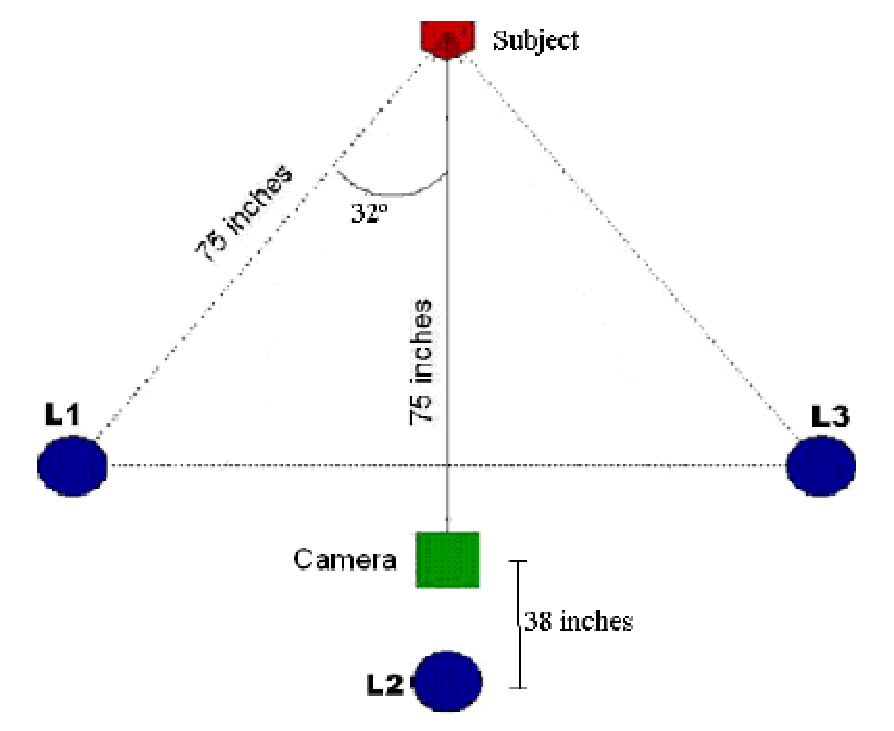
\includegraphics[scale=.5]{yjvcifig0}
% % \caption{Studio setup for capturing face images indoor. Three light
% % sources L1, L2, L3 were used in conjunction with normal office lights.}
% % \end{figure}

% You might find positioning your artwork within the text difficult
% anyway. In that case you may choose to place all artwork at the end of
% the text and insert a marker in the text at the desired place. In any
% case, please keep in mind that the placement of artwork may vary
% somewhat in relation to the page lay-out \cite{HullermeierRifqi2009}.

% This can easily be achieved using \verb+endfloat.sty+ package. Please
% refer the following documentation to use this package.
% \makeatletter
% \if@twocolumn
% \begin{verbatim}
%   http://mirrors.ctan.org/macros/latex/contrib/
%   endfloat/endfloat.pdf
% \end{verbatim}
% \else
% \begin{verbatim}
%   http://mirrors.ctan.org/macros/latex/contrib/endfloat/endfloat.pdf
% \end{verbatim}
% \fi
% \makeatother

% \textcolor{newcolor}{\bf You should insert a caption for the figures
% below the figures and for the tables the caption should be above the
% tables.} 

% Please remember that we will always also need highresolution versions
% of your artwork for printing, submitted as separate files in standard
% format (i.e. TIFF or EPS), not included in the text document. Before
% preparing your artwork, please take a look at our Web page:
% \url{http://www.elsevier.com/locate/authorartwork}.

% \subsection{Lists}

% For tabular summations that do not deserve to be presented as
% a table, lists are often used. Lists may be either numbered or
% bulleted. Below you see examples of both.
% \begin{enumerate}
% \item The first entry in this list
% \item The second entry
% \begin{enumerate}
% \item A subentry
% \end{enumerate}
% \item The last entry
% \end{enumerate}
% \begin{itemize}
% \item A bulleted list item
% \item Another one
% \end{itemize}

% \subsection{Equations}
% Conventionally, in mathematical equations, variables and
% anything that represents a value appear in italics.
% All equations should be numbered for easy referencing. The number
% should appear at the right margin.
% \begin{equation}
% S_{\rm pg}'=\frac{S_{\rm pg}-\min(S_{\rm pG})}
%  {\max(S_{\rm pG}-\min(S_{\rm pG})}
% \end{equation}
% In mathematical expressions in running text ``/'' should be used for
% division (not a horizontal line). 

\section*{Acknowledgments}
Acknowledgments should be inserted at the end of the paper, before the
references, not as a footnote to the title. Use the unnumbered
Acknowledgements Head style for the Acknowledgments heading.

\section*{References}

Please ensure that every reference cited in the text is also present in the
reference list (and vice versa).

\section*{\itshape Reference style}

Text: All citations in the text should refer to:
\begin{enumerate}
  \item Single author: the author's name (without initials, unless there is ambiguity)
        and the year of publication;
  \item Two authors: both authors' names and the year of publication;
  \item Three or more authors: first author's name followed by `et al.' and the year of
        publication.
\end{enumerate}
Citations may be made directly (or parenthetically). Groups of
references should be listed first alphabetically, then chronologically.

%%Harvard
\bibliographystyle{model1-num-names.bst}
\bibliography{refs}

\section*{Supplementary Material}

Supplementary material that may be helpful in the review process should be
prepared and provided as a separate electronic file. That file can then be
transformed into PDF format and submitted along with the manuscript and graphic
files to the appropriate editorial office.

\end{document}

%%
